% Options for packages loaded elsewhere
\PassOptionsToPackage{unicode}{hyperref}
\PassOptionsToPackage{hyphens}{url}
\PassOptionsToPackage{dvipsnames,svgnames,x11names}{xcolor}
%
\documentclass[
  letterpaper,
  DIV=11,
  numbers=noendperiod,
  oneside]{scrartcl}

\usepackage{amsmath,amssymb}
\usepackage{iftex}
\ifPDFTeX
  \usepackage[T1]{fontenc}
  \usepackage[utf8]{inputenc}
  \usepackage{textcomp} % provide euro and other symbols
\else % if luatex or xetex
  \usepackage{unicode-math}
  \defaultfontfeatures{Scale=MatchLowercase}
  \defaultfontfeatures[\rmfamily]{Ligatures=TeX,Scale=1}
\fi
\usepackage{lmodern}
\ifPDFTeX\else  
    % xetex/luatex font selection
\fi
% Use upquote if available, for straight quotes in verbatim environments
\IfFileExists{upquote.sty}{\usepackage{upquote}}{}
\IfFileExists{microtype.sty}{% use microtype if available
  \usepackage[]{microtype}
  \UseMicrotypeSet[protrusion]{basicmath} % disable protrusion for tt fonts
}{}
\makeatletter
\@ifundefined{KOMAClassName}{% if non-KOMA class
  \IfFileExists{parskip.sty}{%
    \usepackage{parskip}
  }{% else
    \setlength{\parindent}{0pt}
    \setlength{\parskip}{6pt plus 2pt minus 1pt}}
}{% if KOMA class
  \KOMAoptions{parskip=half}}
\makeatother
\usepackage{xcolor}
\usepackage[left=1in,marginparwidth=2.0666666666667in,textwidth=4.1333333333333in,marginparsep=0.3in]{geometry}
\setlength{\emergencystretch}{3em} % prevent overfull lines
\setcounter{secnumdepth}{-\maxdimen} % remove section numbering
% Make \paragraph and \subparagraph free-standing
\makeatletter
\ifx\paragraph\undefined\else
  \let\oldparagraph\paragraph
  \renewcommand{\paragraph}{
    \@ifstar
      \xxxParagraphStar
      \xxxParagraphNoStar
  }
  \newcommand{\xxxParagraphStar}[1]{\oldparagraph*{#1}\mbox{}}
  \newcommand{\xxxParagraphNoStar}[1]{\oldparagraph{#1}\mbox{}}
\fi
\ifx\subparagraph\undefined\else
  \let\oldsubparagraph\subparagraph
  \renewcommand{\subparagraph}{
    \@ifstar
      \xxxSubParagraphStar
      \xxxSubParagraphNoStar
  }
  \newcommand{\xxxSubParagraphStar}[1]{\oldsubparagraph*{#1}\mbox{}}
  \newcommand{\xxxSubParagraphNoStar}[1]{\oldsubparagraph{#1}\mbox{}}
\fi
\makeatother


\providecommand{\tightlist}{%
  \setlength{\itemsep}{0pt}\setlength{\parskip}{0pt}}\usepackage{longtable,booktabs,array}
\usepackage{calc} % for calculating minipage widths
% Correct order of tables after \paragraph or \subparagraph
\usepackage{etoolbox}
\makeatletter
\patchcmd\longtable{\par}{\if@noskipsec\mbox{}\fi\par}{}{}
\makeatother
% Allow footnotes in longtable head/foot
\IfFileExists{footnotehyper.sty}{\usepackage{footnotehyper}}{\usepackage{footnote}}
\makesavenoteenv{longtable}
\usepackage{graphicx}
\makeatletter
\def\maxwidth{\ifdim\Gin@nat@width>\linewidth\linewidth\else\Gin@nat@width\fi}
\def\maxheight{\ifdim\Gin@nat@height>\textheight\textheight\else\Gin@nat@height\fi}
\makeatother
% Scale images if necessary, so that they will not overflow the page
% margins by default, and it is still possible to overwrite the defaults
% using explicit options in \includegraphics[width, height, ...]{}
\setkeys{Gin}{width=\maxwidth,height=\maxheight,keepaspectratio}
% Set default figure placement to htbp
\makeatletter
\def\fps@figure{htbp}
\makeatother

\KOMAoption{captions}{tableheading}
\makeatletter
\@ifpackageloaded{caption}{}{\usepackage{caption}}
\AtBeginDocument{%
\ifdefined\contentsname
  \renewcommand*\contentsname{Table of contents}
\else
  \newcommand\contentsname{Table of contents}
\fi
\ifdefined\listfigurename
  \renewcommand*\listfigurename{List of Figures}
\else
  \newcommand\listfigurename{List of Figures}
\fi
\ifdefined\listtablename
  \renewcommand*\listtablename{List of Tables}
\else
  \newcommand\listtablename{List of Tables}
\fi
\ifdefined\figurename
  \renewcommand*\figurename{Figure}
\else
  \newcommand\figurename{Figure}
\fi
\ifdefined\tablename
  \renewcommand*\tablename{Table}
\else
  \newcommand\tablename{Table}
\fi
}
\@ifpackageloaded{float}{}{\usepackage{float}}
\floatstyle{ruled}
\@ifundefined{c@chapter}{\newfloat{codelisting}{h}{lop}}{\newfloat{codelisting}{h}{lop}[chapter]}
\floatname{codelisting}{Listing}
\newcommand*\listoflistings{\listof{codelisting}{List of Listings}}
\makeatother
\makeatletter
\makeatother
\makeatletter
\@ifpackageloaded{caption}{}{\usepackage{caption}}
\@ifpackageloaded{subcaption}{}{\usepackage{subcaption}}
\makeatother
\makeatletter
\@ifpackageloaded{sidenotes}{}{\usepackage{sidenotes}}
\@ifpackageloaded{marginnote}{}{\usepackage{marginnote}}
\makeatother

\ifLuaTeX
  \usepackage{selnolig}  % disable illegal ligatures
\fi
\usepackage{bookmark}

\IfFileExists{xurl.sty}{\usepackage{xurl}}{} % add URL line breaks if available
\urlstyle{same} % disable monospaced font for URLs
\hypersetup{
  colorlinks=true,
  linkcolor={blue},
  filecolor={Maroon},
  citecolor={Blue},
  urlcolor={Blue},
  pdfcreator={LaTeX via pandoc}}


\author{}
\date{}

\begin{document}


\subsection{Introduction}\label{introduction}

This report outlines the methodology behind forecasting the outcome of
the upcoming Icelandic Parliamentary Elections scheduled for November
30th. The forecast is based on a dynamic linear model implemented in
Stan, incorporating polling data over time and adjusting for polling
house effects while accounting for overdispersion.

\subsection{Model Specification}\label{model-specification}

We model the polling percentages for each political party over time
using a dynamic linear model with a Dirichlet-Multinomial observation
component. The model captures the evolution of party support and
accounts for variations between different polling houses.

\subsubsection{Notation}\label{notation}

\paragraph{Input Data}\label{input-data}

\begin{itemize}
\tightlist
\item
  \(P\): Number of political parties \emph{(including the Other
  category)}
\item
  \(T\): Number of time points (dates) at which we have polling data
\item
  \(H\): Number of polling houses
\item
  \(N\): Number of observations (polls)
\item
  \(y_{n,p}\): Count of responses for party \(p\) in poll \(n\)
\item
  \(\Delta_t\): The time difference between polls at \(t-1\) and \(t\)
  in days
\end{itemize}

\paragraph{Parameters}\label{parameters}

\begin{itemize}
\tightlist
\item
  \(\beta_{p,t}\): Latent support for party \(p\) at time \(t\) (for
  \(p = 2,\ldots,P\))
\item
  \(\gamma_{p,h}\): Effect of polling house \(h\) for party \(p\) (for
  \(p = 2,\ldots,P\))
\item
  \(\mu_{\gamma,p}\): Mean house effect for party \(p\)
\item
  \(\sigma_{\gamma,p}\): Scale of house effects for party \(p\)
\item
  \(\sigma_p\): Scale parameter for the random walk of party \(p\)
\item
  \(\phi\): Overdispersion parameter
\end{itemize}

\subsubsection{Dynamic Party Effects}\label{dynamic-party-effects}

The latent support for each party (except the reference category)
evolves over time following a random walk with scaled innovations:

\[
\beta_{p,1} = \beta_{p}^{(0)}, \quad \beta_{p,t} = \beta_{p,t-1} + \sigma_p z_{p,t} \sqrt{\Delta_t} \quad \text{for } t = 2, \dots, T, \quad p=1, \dots, P - 1
\]

where \(z_{p,t} \sim \mathcal{N}(0, 1)\) and \(\sqrt{\Delta_t}\) scales
the innovations according to the time difference between polls.

\subsubsection{Polling House Effects}\label{polling-house-effects}

Polling house effects are modeled hierarchically to account for
systematic biases:

\[
\gamma_{p,1} = 0, \quad \gamma_{p,h} = \mu_{\gamma,p} + \sigma_{\gamma,p} \tilde{\gamma}_{p,h} \quad \text{for } h = 2, \dots, H,
\]

where \(\tilde{\gamma}_{p,h} \sim \mathcal{N}(0, 1)\). The parameters
\(\mu_{\gamma,p}\) and \(\sigma_{\gamma,p}\) control the mean and
variability of polling house effects for each party.

Elections are set to be the first polling house and therefore
\(\gamma_{p,1} = 0\).

\subsubsection{Overdispersion}\label{overdispersion}

To account for overdispersion in the polling data, we introduce an
overdispersion parameter \(\phi\):

\[
\phi = \frac{1}{\phi_{\text{inv}}},
\]

where \(\phi_{\text{inv}} \sim \text{Exponential}(1)\).

\subsection{Data and Likelihood}\label{data-and-likelihood}

The observed counts
\(\mathbf{y}_{n} = \left(y_{n,1}, \dots, y_{n,P}\right)\) are modeled
using a Dirichlet-Multinomial distribution:

\[
\mathbf{y}_{n} \sim \text{Dirichlet-Multinomial}\left(\sum_{p=1}^P y_{n,p}, \phi \cdot \boldsymbol{\pi}_{n}\right),
\]

where
\(\boldsymbol{\pi}_{n} = \text{softmax}\left(\boldsymbol{\eta}_{n}\right)\)
and \(\boldsymbol{\eta}_{n}\) includes the latent support and polling
house effect for each party, with the first party's linear predictor
constrained to be the negative sum of other parties' predictors:

\[
\eta_{n,p} = \begin{cases}
-\sum_{p^*=2}^{P} (\beta_{p^*,t_n} + \gamma_{p^*,h_n}) & \text{if } p = 1 \\
\beta_{p,t_n} + \gamma_{p,h_n} & \text{if } p > 1
\end{cases}
\]

\subsection{Prior Distributions}\label{prior-distributions}

The priors are specified as follows:

\begin{itemize}
\tightlist
\item
  \textbf{Initial Party Effects}:
  \(\beta_{p}^{(0)} \sim \mathcal{N}(0, 1)\)
\item
  \textbf{Random Walk Innovations}: \(z_{p,t} \sim \mathcal{N}(0, 1)\)
\item
  \textbf{House Effect Means}: \(\mu_{\gamma,p} \sim \mathcal{N}(0, 1)\)
  with \(\sum_p \mu_{\gamma,p} \sim \mathcal{N}(0, 1)\)
\item
  \textbf{House Effect Scales}:
  \(\sigma_{\gamma,p} \sim \text{Exponential}(1)\)
\item
  \textbf{Random Walk Scales}: \(\sigma_p \sim \text{Exponential}(1)\)
\item
  \textbf{Overdispersion Parameter Inverse}:
  \(\phi_{\text{inv}} \sim \text{Exponential}(1)\)
\end{itemize}

\subsection{Inference}\label{inference}

Bayesian inference is performed using Markov Chain Monte Carlo (MCMC)
sampling via Stan. Posterior distributions of the latent variables
\(\beta_{p,t}\) and \(\gamma_{p,h}\) are obtained, allowing for
probabilistic forecasting of election outcomes. The overdispersion
parameter \(\phi\) helps in capturing extra variability in the polling
data beyond the multinomial assumption.

\subsection{Posterior Predictive
Checks}\label{posterior-predictive-checks}

To assess the model's fit, posterior predictive simulations are
conducted:

\[
\mathbf{y}_{\text{rep},d} \sim \text{Dirichlet-Multinomial}\left(n_{\text{pred}}, \phi \cdot \boldsymbol{\pi}_{d}\right),
\]

where
\(\boldsymbol{\pi}_{d} = \text{softmax}\left(\boldsymbol{\eta}_{d}\right)\)
and \(\boldsymbol{\eta}_{d}\) is constructed such that its first
component is the negative sum of the remaining components, which are the
latent party support values \(\beta_{p,d}\).

\subsection{Conclusion}\label{conclusion}

The dynamic linear model effectively captures the temporal evolution of
party support and adjusts for polling house biases while accounting for
overdispersion in the data. By leveraging Bayesian methods, we obtain a
comprehensive probabilistic forecast of the election outcomes,
accounting for uncertainty in the estimates.

\section{Results}\label{results}

\begin{figure*}

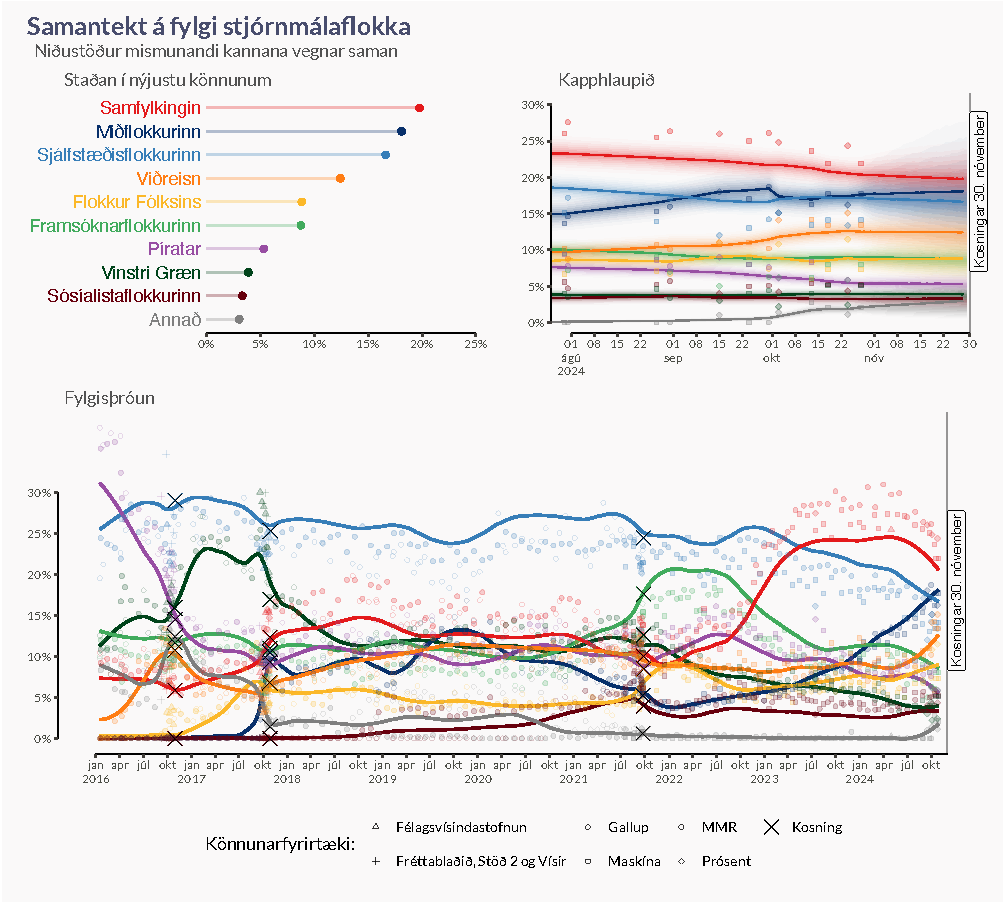
\includegraphics{index_files/figure-pdf/unnamed-chunk-1-1.pdf}

\textsubscript{Source:
\href{https://metill-is.github.io/kosningaspa/index.qmd.html}{Article
Notebook}}

\end{figure*}%




\end{document}
